% IEEE standard conference template; to be used with:
%   spconf.sty  - LaTeX style file, and
%   IEEEbib.bst - IEEE bibliography style file.
% --------------------------------------------------------------------------

\documentclass[letterpaper]{article}
\usepackage{spconf,amsmath,amssymb,graphicx}
\usepackage{graphicx}
\usepackage[export]{adjustbox}


% Example definitions.
% --------------------
% nice symbols for real and complex numbers
\newcommand{\R}[0]{\mathbb{R}}
\newcommand{\C}[0]{\mathbb{C}}

% bold paragraph titles
\newcommand{\mypar}[1]{{\bf #1.}}

% Title.
% ------
\title{Parallel SAT Solving}
%
% Single address.
% ---------------
\name{Jan Eberhardt, Jakub Lichman, Ziwei Huang}
\address{Department of Computer Science\\ ETH Zurich\\Zurich, Switzerland}

% For example:
% ------------
%\address{School\\
%		 Department\\
%		 Address}
%
% Two addresses (uncomment and modify for two-address case).
% ----------------------------------------------------------
%\twoauthors
%  {A. Author-one, B. Author-two\sthanks{Thanks to XYZ agency for funding.}}
%		 {School A-B\\
%		 Department A-B\\
%		 Address A-B}
%  {C. Author-three, D. Author-four\sthanks{The fourth author performed the work
%		 while at ...}}
%		 {School C-D\\
%		 Department C-D\\
%		 Address C-D}
%

\begin{document}
%\ninept
%
\maketitle
%

The hard page limit is 6 pages in this style. Do not reduce font size
or use other tricks to squeeze. This pdf is formatted in the American letter format, so the spacing may look a bit strange when printed out.

\begin{abstract}
Describe in concise words what you do, why you do it (not necessarily
in this order), and the main result.  The abstract has to be
self-contained and readable for a person in the general area. You
should write the abstract last.
\end{abstract}

\section{Introduction}\label{sec:intro}

\mypar{Motivation}


:why it is important? - because it is used it model checking(formal verification), automated planning and scheduling, Combinatorial design and many more. Many problems are transformed into boolean formulas which are than solved with SAT solvers.

:why you are doing? - Current trends in computer hardware design decrease performance per processing unit and pack more units on a single processor. It happened because thermal wall stopped further increase of clock speed. However, algorithms for SAT solving like DPLL and CDCL were invented before wide use of parallelism and therefore were designed for sequential execution. Since SAT is NP-complete problem, it is the right candidate for running it in parallel.

:what are you doing? - In our approach, we are trying to exploit more cores(bring parallelism to SAT solving). This should lead to significant increase of speed and scalability. 

-----------------------------------------------\\

Do not start the introduction with the abstract or a slightly modified
version. It follows a possible structure of the introduction. 
Note that the structure can be modified, but the
content should be the same. Introduction and abstract should fill at most the first page, better less.

\mypar{Motivation} The first task is to motivate what you do.  You can
start general and zoom in one the specific problem you consider.  In
the process you should have explained to the reader: what you are doing,
why you are doing, why it is important (order is usually reversed).

For example, if my result is the fastest sorting implementation ever, one
could roughly go as follows. First explain why sorting is important
(used everywhere with a few examples) and why performance matters (large datasets,
realtime). Then explain that fast implementations are very hard and
expensive to get (memory hierarchy, vector, parallel). 

Now you state what you do in this paper. In our example: 
presenting a sorting implementation that is
faster for some sizes as all the other ones.

\mypar{Related work} Next, you have to give a brief overview of
related work. For a report like this, anywhere between 2 and 8
references. Briefly explain what they do. In the end contrast to what
you do to make now precisely clear what your contribution is.

\section{Background: Whatever the Background is}\label{sec:background}

In this section we are going to have a look at history of SAT solving algorithms as well as new challenges that parallel computing brings to world of SAT solvers. 

SAT solver is program that is able to decide whether given formula is satisfiable i.e. there exists assignment of variables that makes whole formula true-satisfiable or not-unsatisfiable. 
First algorithm was develop in 1960 by Martin Davis and Hilary Putnam for checking the validity of a first-order logic formula using a resolution-based decision procedure for propositional logic.
%[src: https://en.wikipedia.org/wiki/Davis%E2%80%93Putnam_algorithm]. 
Since Davis-Putnam algorithm was able to handle just valid formulas, more general procedure for SAT solving was needed. In 1962 was developed new, complete algorithm that was able to handle all types of formulas. The algorithm is called DPLL after Davis�Putnam�Logemann�Loveland. Its  backtracking-based search algorithm that still forms the basis for most efficient complete SAT solvers. Since DPLL invention there were many algorithms proposed, which improve runtime of SAT solving significantly. 

Give a short, self-contained summary of necessary
background information. For example, assume you present an
implementation of sorting algorithms. You could organize into sorting
definition, algorithms considered, and asymptotic runtime statements. The goal of the
background section is to make the paper self-contained for an audience
as large as possible. As in every section
you start with a very brief overview of the section. Here it could be as follows: In this section 
we formally define the sorting problem we consider and introduce the algorithms we use
including a cost analysis.

\mypar{Sorting}
Precisely define sorting problem you consider.

\mypar{Sorting algorithms}
Explain the algorithm you use including their costs.

As an aside, don't talk about "the complexity of the algorithm.'' It's incorrect,
problems have a complexity, not algorithms.


\section{Your Proposed Method}\label{sec:yourmethod}

Now comes the ``beef'' of the report, where you explain what you
did. Again, organize it in paragraphs with titles. As in every section
you start with a very brief overview of the section.

In this section, structure is very important so one can follow the technical content.

Mention and cite any external resources that you used including libraries or other code.

\section{Experimental Results}\label{sec:exp}

Here you evaluate your work using experiments. You start again with a
very short summary of the section. The typical structure follows.

\mypar{Experimental setup} Specify the platform (processor, frequency, maybe OS, maybe cache sizes)
as well as the compiler, version, and flags used. If your work is about performance, 
I strongly recommend that you play with optimization flags and consider also icc for additional potential speedup.

Then explain what kind of benchmarks you ran. The idea is to give enough information so the experiments are reproducible by somebody else on his or her code.
For sorting you would talk about the input sizes. For a tool that performs NUMA optimization, you would specify the programs you ran.

\mypar{Results}
Next divide the experiments into classes, one paragraph for each. In each class of experiments you typically pursue one questions that then is answered by a suitable plot or plots. For example, first you may want to investigate the performance behavior with changing input size, then how your code compares to external benchmarks.

For some tips on benchmarking including how to create a decent viewgraph see pages 22--27 in \cite{Pueschel:10}.

{\bf Comments:}
\begin{itemize}
\item Create very readable, attractive plots (do 1 column, not 2 column plots
for this report) with readable font size. However, the font size should also not be too large; typically it is smaller than the text font size.
An example is in Fig.~\ref{fftperf} (of course you can have a different style).
\item Every plot answers a question. You state this question and extract the
answer from the plot in its discussion.
\item Every plot should be referenced and discussed.
\end{itemize}

\begin{figure}
  \centering
  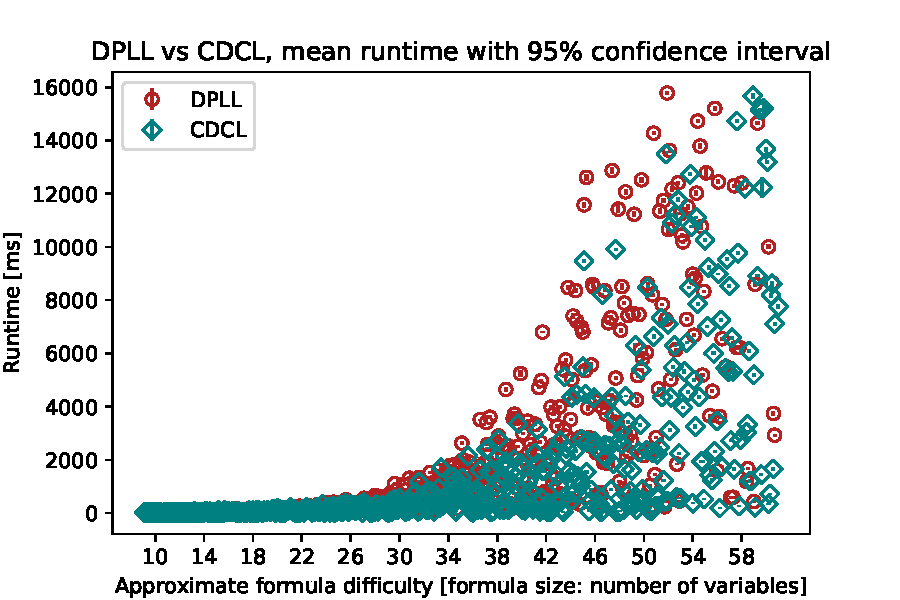
\includegraphics[width=\columnwidth]{figures/dpll_vs_cdcl_scatter}
  \caption{TODO.\label{dpll_vs_cdcl_speedup}}
\end{figure}

\begin{figure}
  \centering
  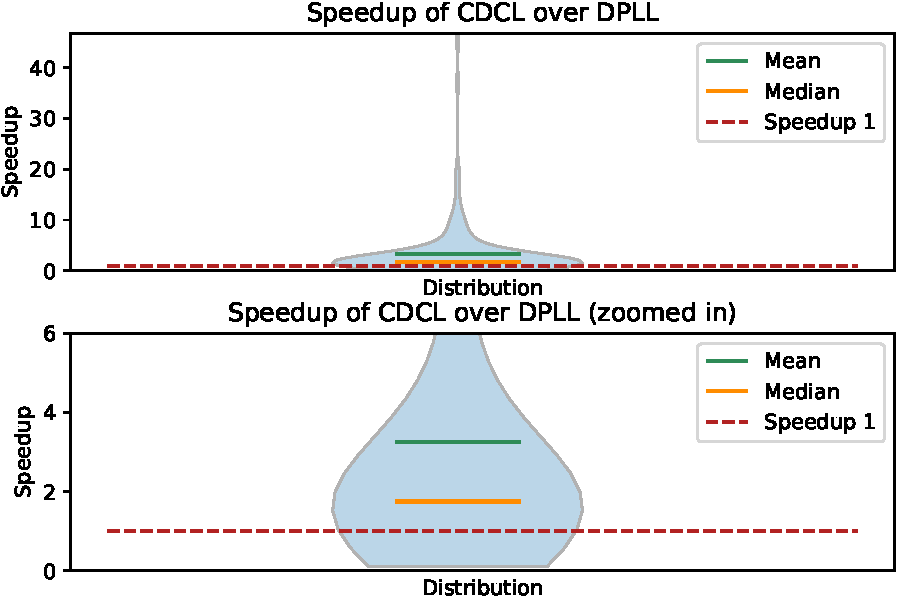
\includegraphics[width=\columnwidth]{figures/dpll_vs_cdcl_speedup}
  \caption{Speedup of CDCL compared to DPLL. Both algorithms were run sequentially.\label{dpll_vs_cdcl_speedup}}
\end{figure}

\begin{figure}
  \centering
  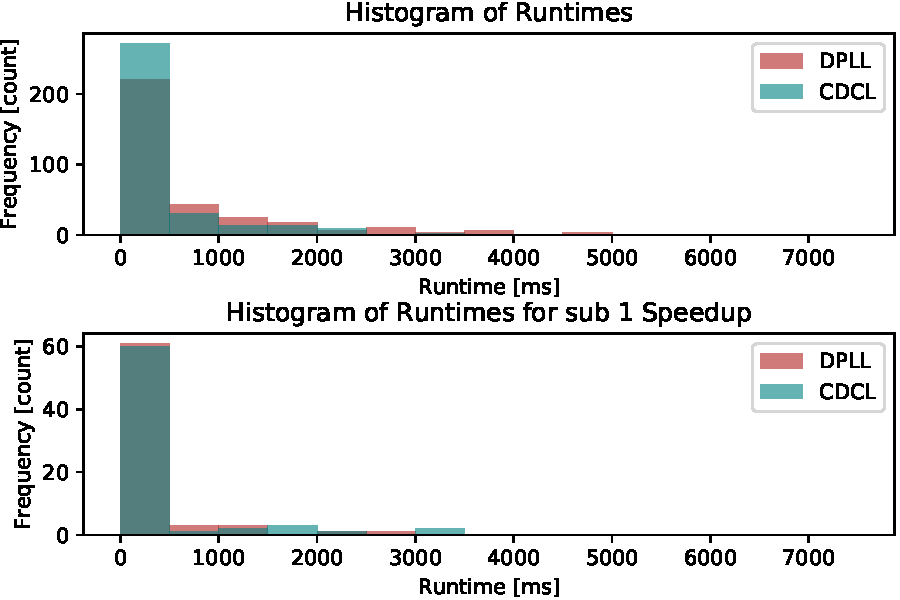
\includegraphics[width=\columnwidth]{figures/dpll_vs_cdcl_histo}
  \caption{TODO.\label{dpll_vs_cdcl_speedup}}
\end{figure}

\section{Conclusions}

Here you need to summarize what you did and why this is
important. {\em Do not take the abstract} and put it in the past
tense. Remember, now the reader has (hopefully) read the report, so it
is a very different situation from the abstract. Try to highlight
important results and say the things you really want to get across
such as high-level statements (e.g., we believe that .... is the right
approach to .... Even though we only considered x, the
.... technique should be applicable ....) You can also formulate next
steps if you want. Be brief. After the conclusions there are only the references.

\section{Further comments}

Here we provide some further tips.

\mypar{Further general guidelines}

\begin{itemize}
\item For short papers, to save space, I use paragraph titles instead of
subsections, as shown in the introduction.

\item It is generally a good idea to break sections into such smaller
units for readability and since it helps you to (visually) structure the story.

\item The above section titles should be adapted to more precisely
reflect what you do.

\item Each section should be started with a very
short summary of what the reader can expect in this section. Nothing
more awkward as when the story starts and one does not know what the
direction is or the goal.

\item Make sure you define every acronym you use, no matter how
convinced you are the reader knows it.

\item Always spell-check before you submit (to us in this case).

\item Be picky. When writing a paper you should always strive for very
high quality. Many people may read it and the quality makes a big difference.
In this class, the quality is part of the grade.

\item Books helping you to write better: \cite{Higham:98} and \cite{Strunk:00}.

\item Conversion to pdf (latex users only): 

dvips -o conference.ps -t letter -Ppdf -G0 conference.dvi

and then

ps2pdf conference.ps
\end{itemize}

\mypar{Graphics} For plots that are not images {\em never} generate the bitmap formats
jpeg, gif, bmp, tif. Use eps, which means encapsulate postscript. It is
scalable since it is a vector graphic description of your graph. E.g.,
from Matlab, you can export to eps.

The format pdf is also fine for plots (you need pdflatex then), but only if the plot was never before in the format 
jpeg, gif, bmp, tif.


% References should be produced using the bibtex program from suitable
% BiBTeX files (here: bibl_conf). The IEEEbib.bst bibliography
% style file from IEEE produces unsorted bibliography list.
% -------------------------------------------------------------------------
\bibliographystyle{IEEEbib}
\bibliography{bibl_conf}

\end{document}

